\section{Analysis}

\label{intro}

\subsection{Race Composition Across Institutions}
Comparing the  \href{https://en.wikipedia.org/wiki/Demographics_of_Florida}{2010 census}  and \href{https://www.census.gov/prod/2002pubs/c2kprof00-fl.pdf}{2000 census} we find 
White-Not Hispanic race proportion dropped from 60\% to 53.5\%, 11\% drop in 10 years.  The white-not Hispanic race proportion in (university, state, city, school teachers, county) has only dropped 4-6\% in the years spanning longer than that period.  Florida public payroll data shows all race is under-represented across (university, state, city, school teachers, county) except for Asians at the university level, which only constitutes 8\% of Florida's public payroll data counts.


\begin{figure}[H]
\begin{center}
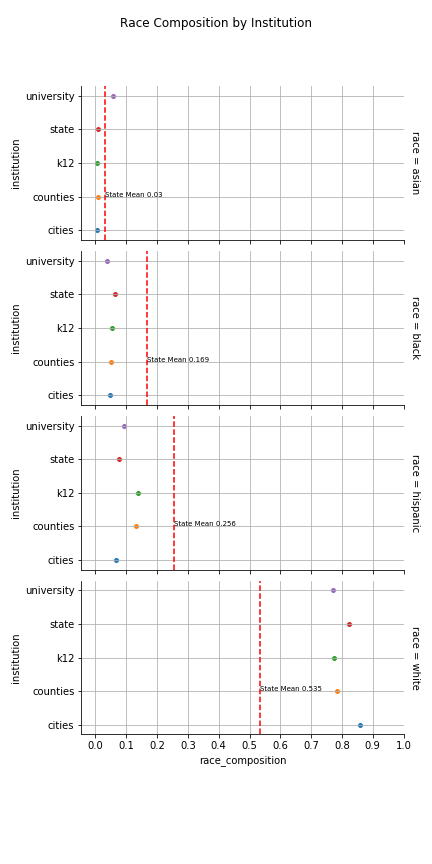
\includegraphics[width=3.5in]{Figures/race_composition_across_inst.png}
\caption{Florida's public sector race composition}
\label{styleResponse}
\end{center}
\end{figure}


\subsection{Institution median pay by race}
fill in


\begin{figure}[H]
\begin{center}
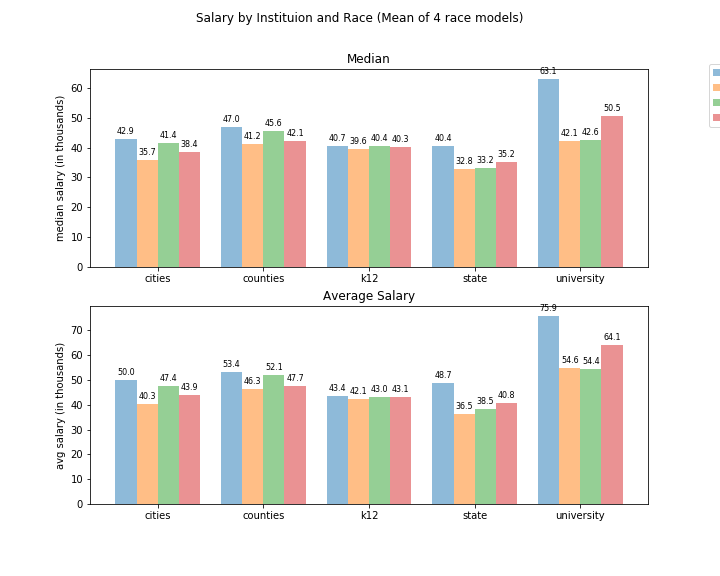
\includegraphics[width=5.5in]{Figures/race_median_pay}
\caption{Median pay of Florida's public sector by race }
\label{styleResponse}
\end{center}
\end{figure}

\subsection{Race Composition Time Series}
fill in


\begin{figure}[H]
\begin{center}
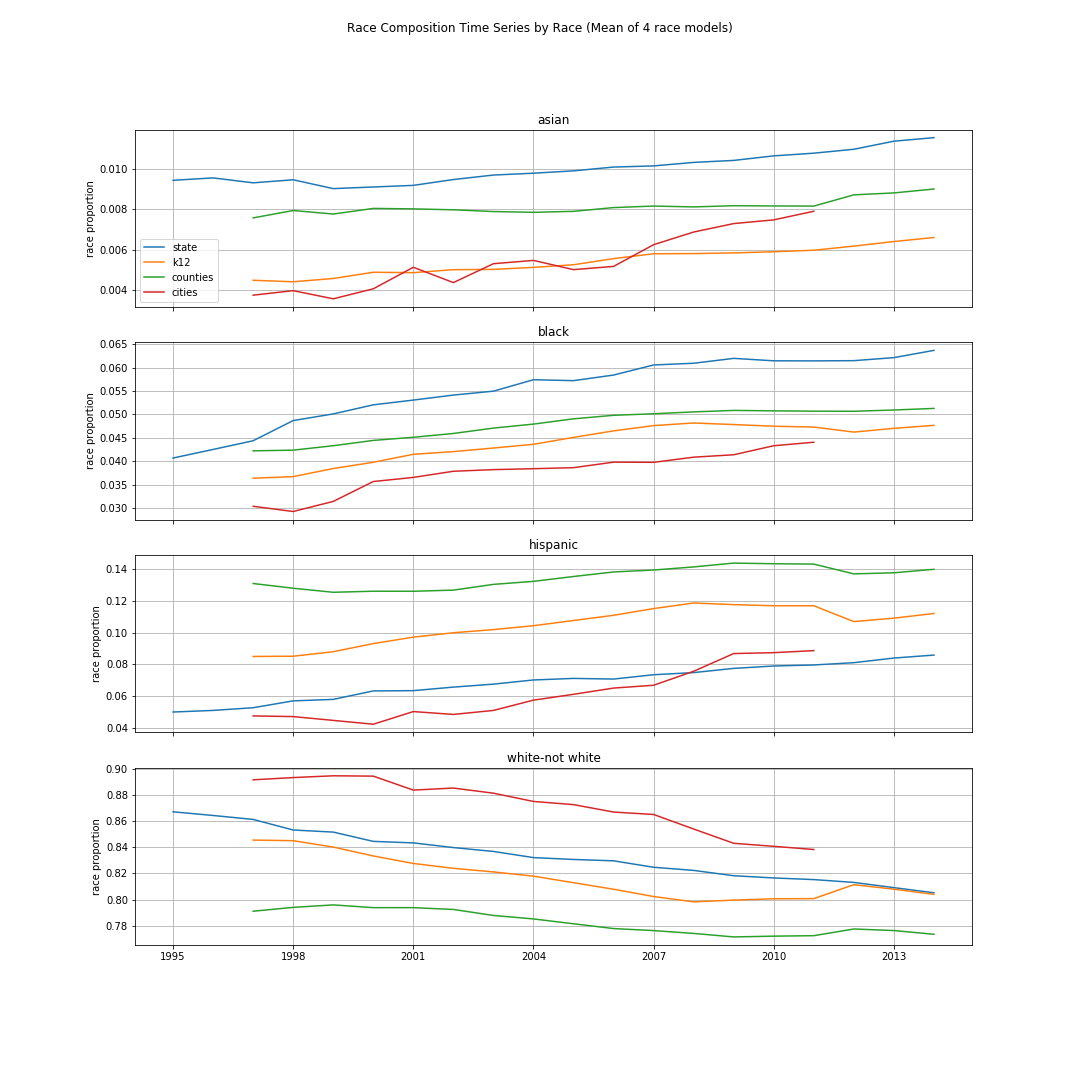
\includegraphics[width=5.5in]{Figures/race_composition_ts.png}
\caption{Time Series: Florida's public sector race composition}
\label{styleResponse}
\end{center}
\end{figure}


\subsection{Race Median Pay Time Series}
fill in


\begin{figure}[H]
\begin{center}
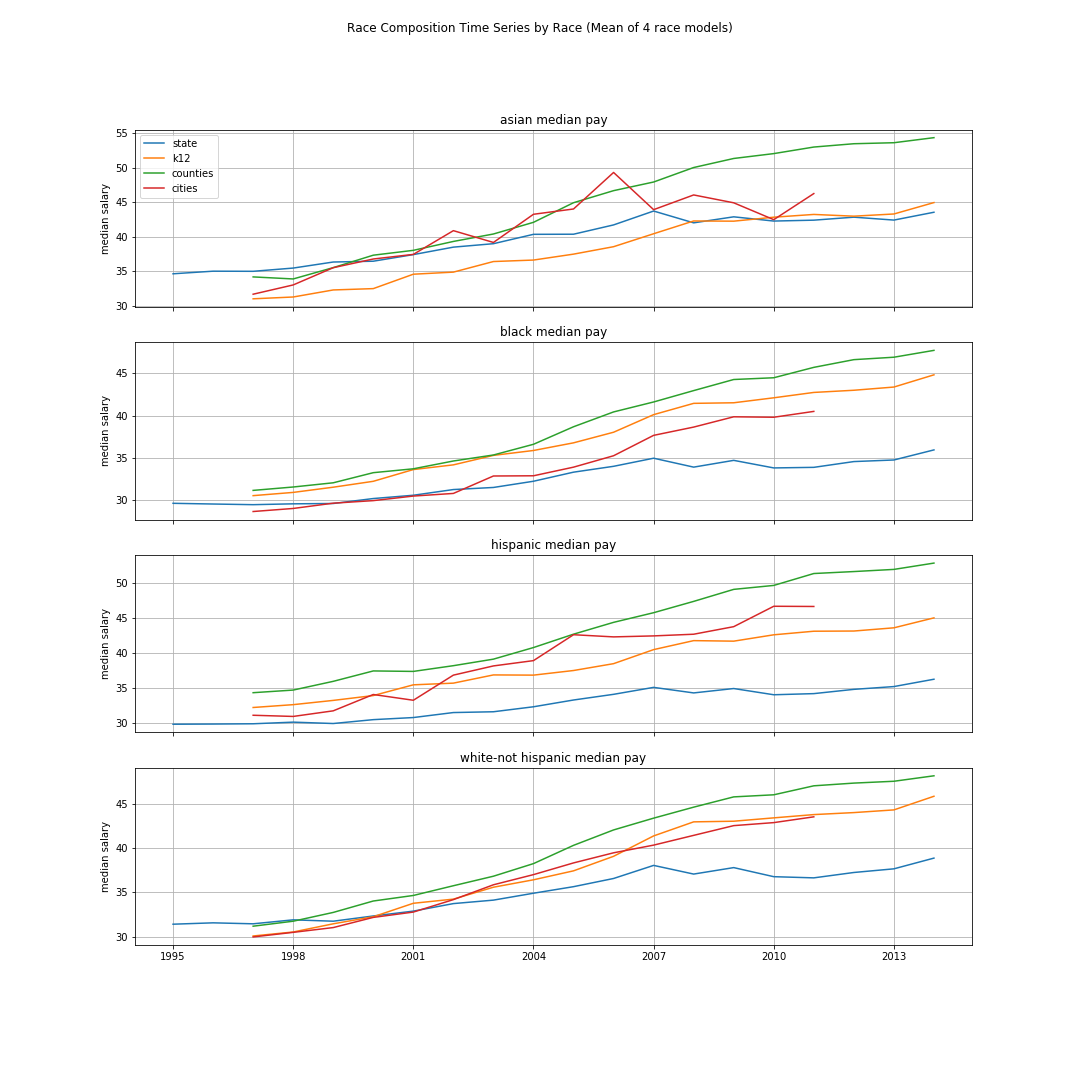
\includegraphics[width=5.5in]{Figures/median_salary_ts.png}
\caption{Time Series: Florida's public sector median pay}
\label{styleResponse}
\end{center}
\end{figure}